% Implementation & validation

The proposed in-system debugger has been implemented for all the AJIT processor models and validated with several test programs. The software subsystem is described in C and the hardware subsystem descriptions are according to the corresponding processor models are designed for.

\section{Implementation}
\subsection{Software subsystem and Debug link}
The cross GDB to be used for debugging the AJIT processor programs is generated by compiling the standard GDB source files with \textit{--target=sparc-buildroot-linux-uclibc} option. It can be invoked by \textit{sparc-linux-gdb} command on the host machine terminal. The source files have to be compiled with the \texttt{gcc}\cite{gcc} cross compiler debug flag (\textit{-g}) to use them for debugging.

In the ISA-C model source code, the software server bridge is referred as GPB (GDB to Processor Bridge). It is implemented as single C thread, compiled to form a library named \textit{gpb}. Later the complete processor executable is created by compiling the core model and linking to this library. Currently the software subsystem supports only one RSP interface, the unix sockets. Functions in \textit{StartGPBThreads.c} initializes everything and starts the main thread,  \textit{gpb.c} contains the main thread that listens on the socket and carries out the all the functionalities. \textit{GDBtoAJITbridge.c} contains all the functions necessary to communicate over RSP interface (GDB to Server bridge) and debug link (Server to Processor). The implementation uses two data structures, one for representing RSP commands (\textit{rsp\_cmd}) and other for representing the debug link commands (\textit{dbg\_cmd}). All the standard functions required for threads and socket communications are used from the \texttt{gcc} libraries.

The current implementation supports only a single type of connection for the debug link, the AHIR-V2 \cite{AhirThesis} pipes. \textit{ENV\_to\_AJIT\_debug\_command} and \textit{AJIT\_to\_ENV\_debug\_response} are the two 32-bit pipes used to communicate with the AJIT processor hardware. A pipe is just essentially a FIFO with handshaking signals that provide a blocking nature to the data transfer\cite{sarath}. They can be used for inter-thread communication in multi-threaded programs. A read request for a pipe will not succeed before some data is written to it and vice-versa. AHIR-V2 provides special read and write functions to facilitate this behaviour. Since the execution is blocked while expecting some data on a pipe, this can also be used as a locking mechanism. This is kind of a hardware mutex similar to those used in software (mutex functions in \texttt{pthread} library).

% Hardware subsystem
\subsection{Debugging on ISA-C model}
Each block of the ISA-C model is described as a thread, and so is the hardware server. It has three main functional blocks : for handling debug link communications, the processor side communication and a core unit to execute the commands sent by software server bridge. Processor core ISA-C model files (\textit{sparcCore.c}, \textit{execute.c}) are modified to achieve the required control flow.

Processor and hardware server use request-acknowledge mode communication through unidirectional AHIR-V2 pipes. When the processor needs to communicate something, it sends the corresponding opcode through \textit{CPU\_HWSERVER\_id} (8-bit pipe) and the current processor state pointer through \textit{CPU\_to\_HWSERVER\_state} (64-bit pipe). The received pointer is used by the hardware server to modify the processor state. Hardware server uses \textit{HWSERVER\_to\_CPU} (32-bit pipe) for sending messages back to the processor pipeline. 

The processor core, hardware server and testbench are compiled together to form a single executable. The memory map of the program and the unix socket port number should be given for running the executable and starting a debug session.

\subsection{Debugging on micro-architecture simulation model}
The micro-architecture model is described in Aa\cite{aaLRM} language, representing the actual hardware of AJIT processor. Even though it is an intermediate representation in the AHIR-V2 toolchain, it can be also used to describe hardware. Such representations could be converted into C language for verification and to VHDL for hardware realization by the AHIR-V2 compiler. It supports the use of same software testbench for hardware and software simulations.

The model has an elastic pipeline with and all the modules are interconnected by AHIR-V2 pipes.
Currently the processor core is described in hardware and the memory and caches are the same ones used with ISA-C model. There are basically two simulation models derived from the micro-architecture Aa description : C, and VHDL. The C code generated from the Aa representation can be compiled together with the testbench to produce a single executable similar to the ISA-C model. The usage and everything else remains the same as the ISA-C model.

The second derived model is by the simulation of generated VHDL description using ModelSim\footnote{http://www.model.com/}. It simulates the core processor module and the testbench connects through the VHPI (VHDL Procedural Interface) library provided by AHIR-V2. The system will behave just like the actual hardware would, and provides a good platform for design verification before moving to hardware.

\subsection{Debugging on micro-architecture FPGA prototype}
The VHDL description generated by AHIR compiler is synthesis ready. The design is synthesized with Vivado\textsuperscript{\textregistered} Design suite and loaded on to the Xilinx\footnote{http://www.xilinx.com/} Virtex-7 VC709 FPGA card. The complete processor hardware with included debug units run at 100MHz on this FPGA prototype.

The communication medium between the testbench and processor hardware is different when it is on the FPGA. The physical interface will be the PCI Express bus, and necessary framework is provided by RIFFA 2.2 (\textbf{R}eusable \textbf{I}ntegration \textbf{F}ramework for \textbf{F}PGA \textbf{A}ccelerators)\cite{riffaPaper} platform. This open source framework provides additional hardware modules and software drivers for synchronizing and communicating FPGA based applications with computers. The complete system architecture of the FPGA prototype with RIFFA is given in Figure \ref{FPGA}.

% Final figure
\begin{figure}[h!]
	\centering
	\def\svgwidth{0.6\columnwidth}
	\import{Figs/FPGA/}{FPGA.tex}
	\caption{In-system debugger on FPGA prototype}
	\label{FPGA}
\end{figure}

The software server bridge and the GDB communicate through RSP interface as described in the previous section. The server bridge and testbench interact through the same AHIR-V2 pipes as mentioned before. Here the testbench use RIFFA drivers for communicating with FPGA PCI Express block. The RIFFA module in hardware will interface this block with the actual AJIT processor with in-built debug modules.

\subsection{AHIR-V2}
AHIR (\textbf{A} \textbf{H}ardware \textbf{I}ntermediate \textbf{R}epresentation) compiler\cite{AhirThesis} is the high level synthesis tool set developed at IIT-Bombay. Systems can be described in higher level languages like C/C++ as algorithms and then converted into VHDL digital system descriptions using the AHIR toolchain.

AHIR tools has a two level approach for this high level synthesis process. First it converts the code written in the higher level language to byte code using LLVM\footnote{http://llvm.org/} compiler. The byte code is subsequently converted into an intermediate representation called \textit{Ahir Assembly} (Aa) language that uses petri nets as the basic data structure mechanism. The Aa representation is optimized and later transformed into VHDL through one more intermediate representation called \textit{Virtual Circuit} (vC). Along with this the compiler also allows conversion of Aa representations into C for the easiness of design verification. The complete design flow is shown in Figure \ref{ahirFlow}. AHIR factorizes any system into three components: control path, data path and storage. AHIR framework and methodology is correct by construction. i.e., the hardware produced from the high level language is the exact functional transformation of the input.

\tikzstyle{int}=[draw, minimum size=1.5cm]
\tikzstyle{init} = [pin edge={thick,black}]

\begin{tikzpicture}[node distance=3.5cm,auto,>=latex']
\node [int] (a) {C};
\node [int, right of=a] (b) {C bytecode};
\node [above =1cm of b] (dummy) {$Aa2C$};
\node [int, right of=b, node distance=4cm] (c) {Aa};
\node [int, right of=c] (d) {vC};\\
\node [int, right of=d] (e) {VHDL};


\path[->] (a) edge node {$llvm$} (b);
\path[->] (b) edge node {$llvm2aa$} (c);
\draw[->] (c) edge node {$Aa2VC$} (d) ;
\draw[->] (d) edge node {$vc2vhdl$} (e) ;

\draw (c.north) |-  (dummy.east);
\draw[->] (dummy.west) -| (a.north) ;
\end{tikzpicture}
\captionof{figure}{AHIR flow}
\label{ahirFlow}

\section{Usage and Validation}
\subsection{Using in-system debugger}
The program for debugging has to be compiled using \texttt{sparc-linux-gcc} cross compiler with \textit{-g} flag for including the debug information. Then the \texttt{sparc-linux-gdb} has to be invoked by providing this executable as the first argument. Now the appropriate testbench has to be started by providing the memory map (generated using the same compiler) of the same program and the port for the debugger to connect. These testbenches could correspond to any of the four AJIT processor models available
\begin{itemize}
	\item ISA-C model
	\item Micro-architecture model in C
	\item Micro-architecture VHDL model running in simulator
	\item Micro-architecture model on FPGA prototype
\end{itemize}

If the model is running on simulator, it has to be started separately. The user will now be able to connect to the AJIT processor from the GDB using the following command.
\begin{lstlisting}[language=bash]
(gdb) target remote :<port number>
\end{lstlisting}
The debugging session of AJIT processor has now been started, and the users can continue using it as a regular GDB session.

\subsection{Validation on FPGA prototype}
Several test programs running on the AJIT processor FPGA hardware prototype are were debugged using this in-system debugger to validate the current implementation.  
 
\vspace{0.5em}
\forceindent An example session of in-system debugging is shown in Figure \ref{GDBsession}. This indicates how the users will be able to use this infrastructure with the simple interface of GDB. Each of these commands from the user passes through all the blocks described in previous section and gathers its response from hardware. The interactions between the host PC and the hardware for this particular example program is shown in Figure. Reading the hardware state is carried out using several commands and their responses probing all the internal registers, few memory addresses and debug registers.

In cases of traps and interrupt, the details about the type of trap and the interrupt level will not provided by the current implementation. The user has to keep their track by adding breakpoints in the corresponding interrupt and trap handlers.

% working screenshot
\begin{figure}[H]
	\centering
	\begin{subfigure}{\textwidth}
		\centering
		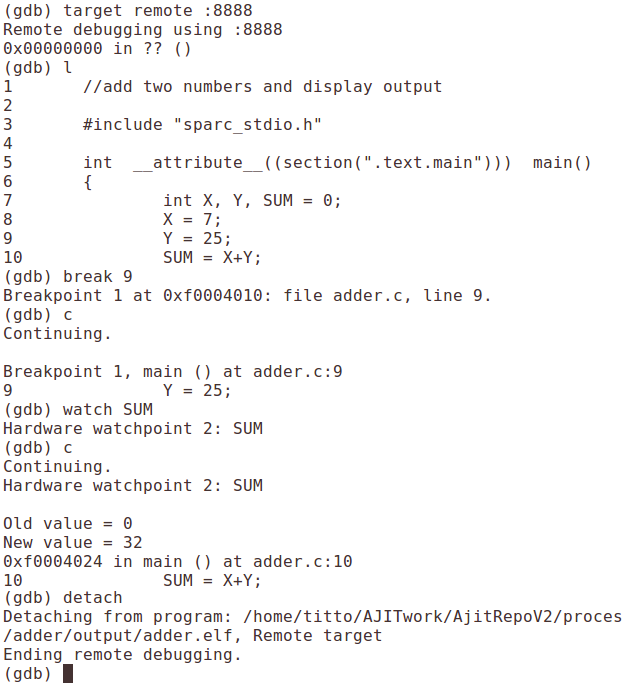
\includegraphics[width=0.8\columnwidth]{Figs/Screenshot/screen.png}
		\subcaption{GDB debug session}
	\end{subfigure}
\end{figure}

\vspace*{4cm}

\begin{figure}[H]
	\ContinuedFloat 	
	\begin{subfigure}{\textwidth}
		\centering
		\def\svgwidth{0.5\columnwidth}
		\import{Figs/SessionComm/}{SessionComm.tex}
		\subcaption{Message communication with hardware}
	\end{subfigure}

	\caption{Validation on FGPA prototype}
	\label{GDBsession}
\end{figure}

Following set of features have been validated on the FPGA prototype and all the previous models with several test programs.
\begin{itemize}
	\item Stop initially and establish connection with GDB
	\item Read/modify the processor register and memory contents
	\item Set/clear break-points/watch-points and stop execution when they are hit
	\item Continue execution indefinitely or single step as per user command
	\item Interrupt the processor execution at any instant 
	\item Detach the debugger and allow normal execution to continue
\end{itemize}